\section{Мета роботи}
Отримати та закріпити знання про внутрішнє (комп’ютерне)
подання числових типів даних у мовах програмування.\\

\noindent
\textbf{Теми для попередньої роботи:}
\begin{itemize}
    \item інформація та її подання в ЕОМ;
    \item адресація пам’яті;
    \item числові типи даних: цілі та дійсні;
    \item похибки подання дійсних чисел;
    \item статичні структури даних – масиви.
\end{itemize}



\section{Завдання}
Написати програму, яка виводить на екран внутрішнє (комп’ютерне)
подання даних чотирьох типів. Типи даних обрати за табл. 3.1 згідно із своїм
номером у журналі групи. Тип елементів масиву обрати за своїм розсудом.

За результатами роботи підготувати звіт з лабораторної роботи, де
навести отримані результати та дати щодо них пояснення, зробити
висновки.

\begin{figure}[h!]
    \centering
    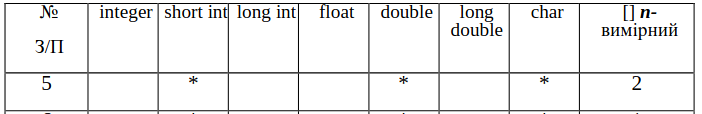
\includegraphics[width=.9\textwidth]{\reportDirectory/var.png}
    \caption{Завдання за варіантом (\variant)}
    \label{fig:task}
\end{figure}


\section{Хід виконання}
Для виконання завдання було обрано мову Rust.
Увесь код також додатково був розміщений в GitHub репозитарії: \href{https://github.com/blackgolyb/algos-labs}{https://github.com/blackgolyb/algos-labs}.


\newpage
\subsection{Підготовка до виконнаня завдання}
Для початку напишемо утилітарні функції для відображення структур даинх в бітовому вигляді та одразу використаємо їх для простих типів даних.
Для цього напишемо:
\begin{itemize}
    \item функцію для виводу байтів та бітів певного вказівника
    \item trait \textit{ShowBytes}, який треба реалізувати для типів даних, які будуть підтримувати вивід в байтовому форматі
    \item макрос для зручногї реалізації трейта \textit{ShowBytes} для простих типів даних
\end{itemize}

\noindent
Код програм алгоримта:
\begin{lstlisting}[language=Rust, style=colouredRust]
pub fn print_raw_bytes(byte: usize, size: usize) {
    print_bytes(&byte as *const usize as *const u8, size);
}

pub fn print_byte(ptr: *const u8) {
    let byte = unsafe { *ptr };
    for j in 0..8 {
        print!("{}", (byte >> (7 - j)) & 1);
    }
}

pub fn print_bytes(ptr: *const u8, size: usize) {
    for i in 0..(size - 1) {
        print_byte(unsafe { ptr.add(i) });
        print!(" ");
    }

    if size > 0 {
        print_byte(unsafe { ptr.add(size - 1) });
    }
}

pub fn show<T>(value: &T) {
    let size = size_of::<T>();
    let ptr = value as *const T as *const u8;
    print_bytes(ptr, size);
}

pub trait ShowBytes {
    fn show_bytes(&self);
}

#[macro_export]
macro_rules! impl_show_bytes {
    ($impl_type:ident) => {
        impl ShowBytes for $impl_type {
            fn show_bytes(&self) {
                show::<$impl_type>(&self);
            }
        }
    };
}

impl_show_bytes!(i8);
impl_show_bytes!(i16);
impl_show_bytes!(i32);
impl_show_bytes!(i64);
impl_show_bytes!(i128);

impl_show_bytes!(u8);
impl_show_bytes!(u16);
impl_show_bytes!(u32);
impl_show_bytes!(u64);
impl_show_bytes!(u128);

impl_show_bytes!(f32);
impl_show_bytes!(f64);

impl_show_bytes!(usize);
impl_show_bytes!(bool);
\end{lstlisting}

\noindent
Також реалізуємо функіцю для зручного тестування працездатності виводу байтів
\begin{lstlisting}[language=Rust, style=colouredRust]
fn test_value<T: FromStr + Display + ShowBytes>(prompt: &str) {
    let mut buffer = String::new();
    print!("{prompt}");
    io::stdout().flush().unwrap();
    io::stdin().read_line(&mut buffer).unwrap();
    match buffer.trim().parse::<T>() {
        Ok(value) => {
            println!("Entered value: {value}");
            print!("Bin: ");
            value.show_bytes();
            println!();
        }
        Err(_) => eprintln!("Error parsing input: {buffer}"),
    }
}
\end{lstlisting}



\newpage
\subsection{Подання \textit{short int}}
Через те, що в Rust трохи інші назви для типів, то \textit{short int} називається \textit{i16}.
В минулому пункті ми вже реалізували логіку представлення байтів тому просто скористаємося нею

\begin{figure}[h!]
    \centering
    
\includegraphics[width=.9\textwidth]{\reportDirectory/short_int.png}
    \caption{Приклад роботи для \textit{short int}}
    \label{fig:task}
\end{figure}


\subsection{Подання \textit{double}}
Через те, що в Rust інші назви для типів, то \textit{double} називається \textit{f64}.
В минулому пункті ми вже реалізували логіку представлення байтів тому просто скористаємося нею

\begin{figure}[h!]
    \centering
    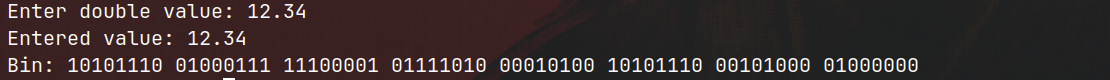
\includegraphics[width=.9\textwidth]{\reportDirectory/double.png}
    \caption{Приклад роботи для \textit{double}}
    \label{fig:task}
\end{figure}


\subsection{Подання \textit{char}}
Напишемо реалізацію трейту \textit{ShowBytes} для \textit{char}
\begin{lstlisting}[language=Rust, style=colouredRust]
impl ShowBytes for char {
    fn show_bytes(&self) {
        let s = self.to_string();
        let bytes = s.as_bytes();
        for byte in bytes {
            print_byte(byte);
        }
        println!();
    }
}
\end{lstlisting}

\begin{figure}[h!]
    \centering
    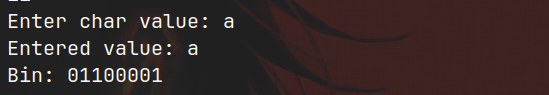
\includegraphics[width=.9\textwidth]{\reportDirectory/char.png}
    \caption{Приклад роботи для \textit{char}}
    \label{fig:task}
\end{figure}


\newpage
\subsection{Подання \textit{Vec}}
Для цього завдання було цікаво дослідити як в Rust працює стандартний \textit{Vec}, який є динамічним масивом.
А також було цікаво реалізувати можливисть робити n-вимірного вектора.

Для початку давайте розгянемо як представляється \textit{Vec} в пам'яті
Як можна побачити нижче, то \textit{Vec} має такі поля: len, cap, ptr.
Також додатково наведемо бінарне представлення усіх його полів, його адресу, розмір в байтах
та бінарне представлення його вмісту.
\begin{figure}[h!]
    \centering
    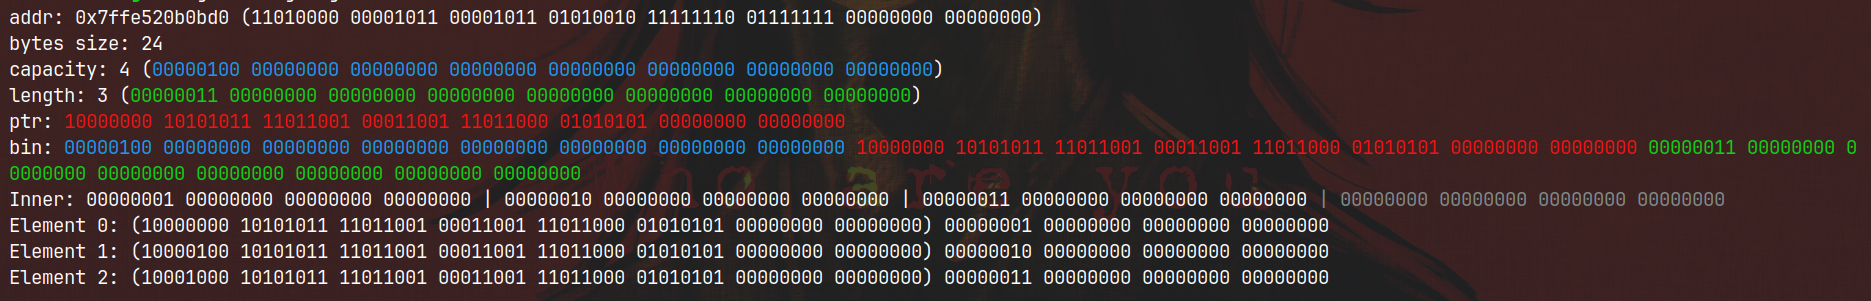
\includegraphics[width=.9\textwidth]{\reportDirectory/vec1.png}
    \caption{Представлення \textit{Vec} у памяті}
    \label{fig:task}
\end{figure}

Далі з цього малюнку можна побачити, що бінарне відображення працює правильно,
бо бінарне представлення вмісту \textit{Vec} співпадає з його бінарним представленням кожного елемента.
Також можна побачити, що \textit{Vec} виділив більше пам'яті ніж треба,
що і відповідає значенню \textit{capacity}.
Не використана пам'ять позначена сірим кольором.
\begin{figure}[h!]
    \centering
    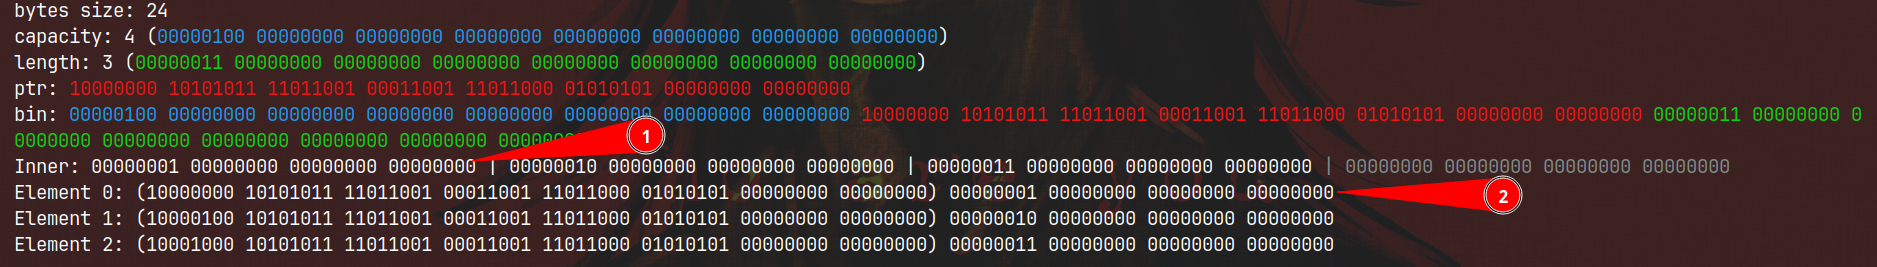
\includegraphics[width=.9\textwidth]{\reportDirectory/vec2.png}
    \caption{Представлення \textit{Vec} у памяті}
    \label{fig:task}
\end{figure}

Також можна побачити, що воно працює правильно,
бо адреса першого елемента масиву співпадає з вказівником в \textit{Vec},
а адреси елементів відрізнаються один від одного на розмір елемента.

\begin{figure}[h!]
    \centering
    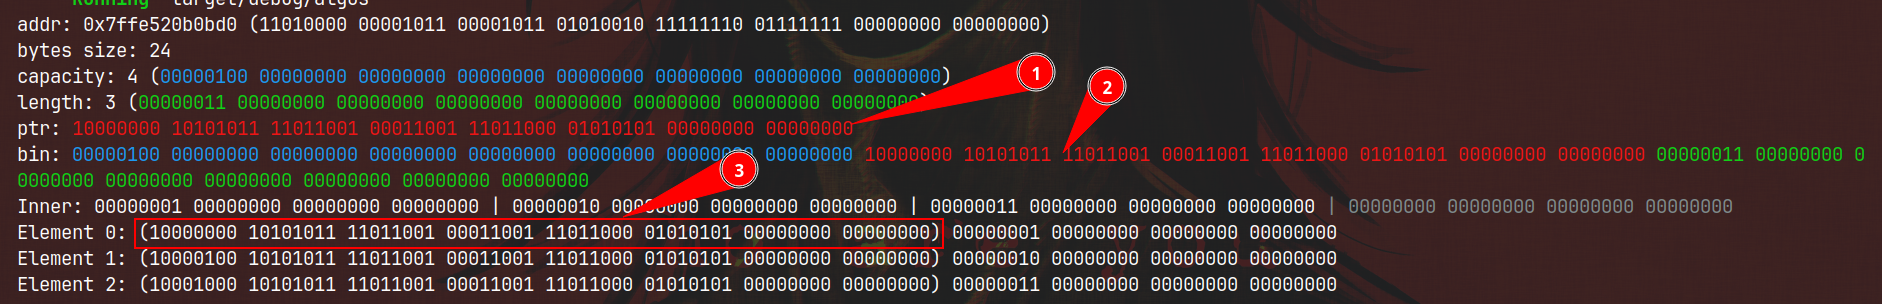
\includegraphics[width=.9\textwidth]{\reportDirectory/vec3.png}
    \caption{Представлення \textit{Vec} у памяті}
    \label{fig:task}
\end{figure}

\begin{figure}[h!]
    \centering
    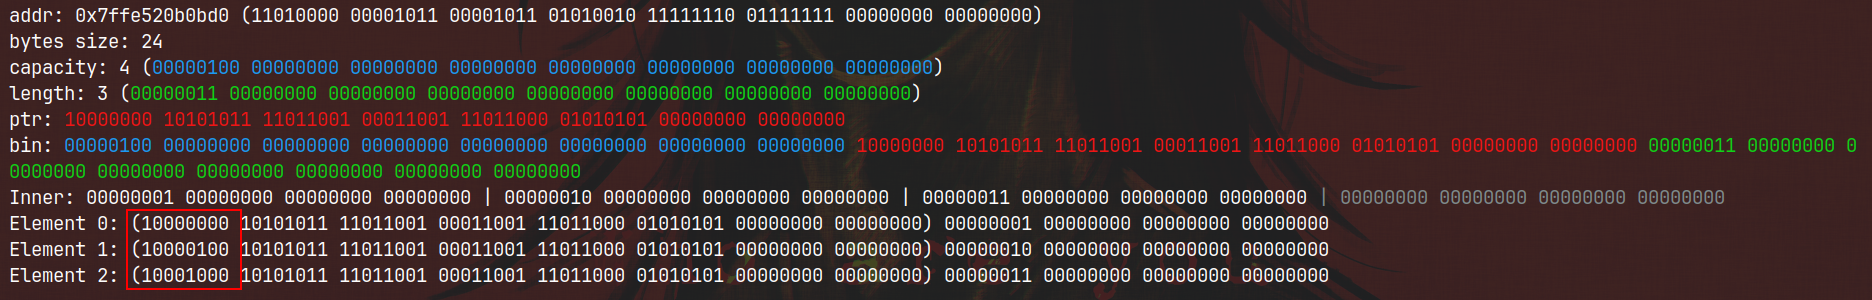
\includegraphics[width=.9\textwidth]{\reportDirectory/vec4.png}
    \caption{Представлення \textit{Vec} у памяті}
    \label{fig:task}
\end{figure}



\newpage
\subsection{Подання \textit{ParsedItem}}
Тепер ми можемо зробити таку структуру, яка буде багатовимірним масивом.
Для цього можна зробити enum, який буде зберігати: або значення, або набір значень.

Напишемо реалізцію його та подивимося, як він виглядає з середини.
\textit{ParsedVec розглянемо пізніше, тому поки можна вважити, що там звичайний Vec.}
\begin{lstlisting}[language=Rust, style=colouredRust]
#[derive(Debug)]
pub enum ParsedItem<T> {
    NestedVec(ParsedVec<T>),
    Value(T),
}

fn test_item() {
    let mut vec = Vec::new();
    vec.push(1);
    vec.push(2);
    vec.push(3);
    let p1: ParsedItem<u32> = ParsedItem::Value(!0);
    let p2: ParsedItem<u32> = ParsedItem::NestedVec(vec.into());
    println!("ParsedItem<u32>: {}   u32: {}\n", size_of::<ParsedItem<u32>>(), size_of::<u32>());

    let size = size_of::<ParsedItem<u32>>();
    print!("ParsedItem::Value: ");
    print_bytes(&p1 as *const ParsedItem<u32> as *const u8, size);
    println!("\n");
    print!("ParsedItem::NestedVec: ");
    print_bytes(&p2 as *const ParsedItem<u32> as *const u8, size);
    println!("\n");
}
\end{lstlisting}


Як можна побачити, то розмір enum в Rust обирається за більшим типом який там є.
А також додаткове місце, якщо воно потрібно на розміщення дискримінант за яким Rust визначає який тип зараз лежить в enum.

В нашому ж випадку Rust не потрібно додаткове місце в силу його внутрішніх оптимізацій.
Тому наш enum буде займати всього 24 байти, що і відповідає розміру \textit{Vec}, тому щоб подивитися що саме та як лежить в нашому enum ми можемо вивести бінарне представлення різних значень цього enum.

Тому для значення enum Value пропоную розглянути інвертований 0, щоб побачити де саме зберігається саме значення,
а для значення enum NestedVec можем взяти вектор з поперднього прикладу, щоб ми могли його легше перевірити
\begin{figure}[h!]
    \centering
    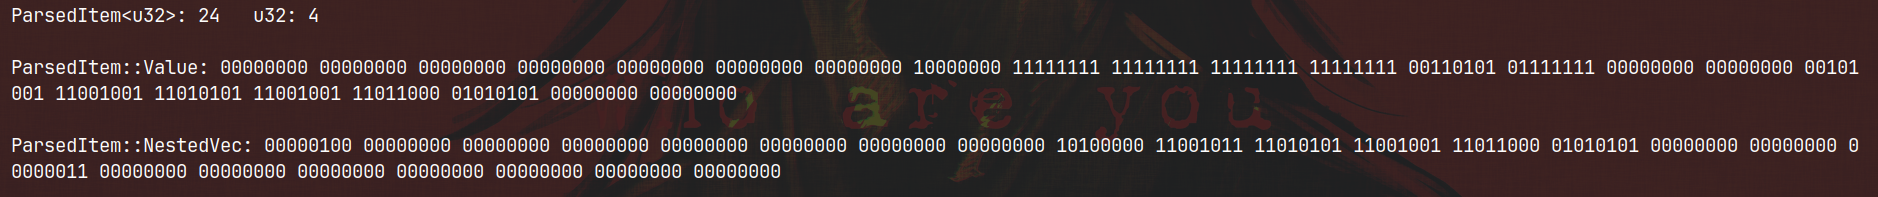
\includegraphics[width=.9\textwidth]{\reportDirectory/parsed_item.png}
    \caption{Представлення \textit{Vec} у памяті}
    \label{fig:task}
\end{figure}


\newpage
\subsection{Подання \textit{ParsedVec}}
Тепер допишемо попередню структуру для того, щоб вона працювала правильно.
\begin{lstlisting}[language=Rust, style=colouredRust]
#[derive(Debug)]
pub enum ParsedItem<T> {
    NestedVec(ParsedVec<T>),
    Value(T),
}

#[derive(Debug)]
pub struct ParsedVec<T>(Vec<ParsedItem<T>>);

impl<T> From<Vec<T>> for ParsedVec<T> {
    fn from(value: Vec<T>) -> Self {
        let mut res = ParsedVec(Vec::new());
        for v in value {
            res.0.push(ParsedItem::Value(v))
        }
        res
        // зроблено так щоб Rust не зміг тут оптимізувати копіювання вектора
        // ParsedVec(value.into_iter().map(|v| ParsedItem::Value(v)).collect())
    }
}
\end{lstlisting}


\newpage
\subsection{Парсинг \textit{ParsedVec}}
Тепер пропоную додати нашій структурі можливість парситися зі строки.
Для цього напишемо парсер, який реалізує trait FromStr для нашої структури \textit{ParsedVec}.
\begin{lstlisting}[language=Rust, style=colouredRust]
#[derive(Debug, PartialEq, Eq)]
pub struct ParseVecError;

impl<T: FromStr + Debug> FromStr for ParsedVec<T>
where
    T::Err: std::fmt::Debug,
{
    type Err = ParseVecError;

    fn from_str(s: &str) -> Result<Self, Self::Err> {
        let s = s
            .trim()
            .strip_prefix('[')
            .and_then(|s| s.strip_suffix(']'))
            .and_then(|s| Some(s.trim()))
            .ok_or(ParseVecError)?;

        let mut items = Vec::new();

        // for empty list/sublist []
        if s.trim().is_empty() {
            return Ok(ParsedVec(items));
        }

        let mut is_err = false;
        for token in s.split(',') {
            let parsed = token.trim().parse::<T>();
            match parsed {
                Err(_) => {
                    is_err = true;
                    break;
                }
                Ok(val) => items.push(ParsedItem::Value(val)),
            }
        }

        if !is_err {
            return Ok(ParsedVec(items));
        }

        let mut items = Vec::new();
        let mut depth = 0;
        let mut start = 0;
        let mut i = 0;
        let mut is_comma = true;
        let mut is_value = false;

        while i < s.len() {
            match &s[i..=i] {
                "[" => {
                    if depth == 0 {
                        if !is_comma {
                            return Err(ParseVecError);
                        }
                        is_comma = false;
                        start = i;
                    }
                    depth += 1;
                }
                "]" => {
                    if depth == 1 {
                        let parsed = s[start..=i].parse::<ParsedVec<T>>()?;
                        items.push(ParsedItem::NestedVec(parsed));
                    }
                    depth -= 1;
                }
                "," if depth == 0 => {
                    if is_comma {
                        return Err(ParseVecError);
                    }
                    if is_value {
                        let parsed = s[start..i].trim().parse::<T>();
                        if parsed.is_err() {
                            return Err(ParseVecError);
                        }
                        is_value = false;
                        items.push(ParsedItem::Value(parsed.unwrap()));
                    }
                    is_comma = true;
                }
                " " => (),
                "\n" => (),
                "\t" => (),
                _ if depth == 0 && is_comma && !is_value => {
                    is_value = true;
                    is_comma = false;
                    start = i;
                }
                _ => (),
            }
            i += 1;
        }

        if is_value {
            let parsed = s[start..].trim().parse::<T>();
            if parsed.is_err() {
                return Err(ParseVecError);
            }
            items.push(ParsedItem::Value(parsed.unwrap()));
        }

        Ok(ParsedVec(items))
    }
}    
\end{lstlisting}

\begin{figure}[h!]
    \centering
    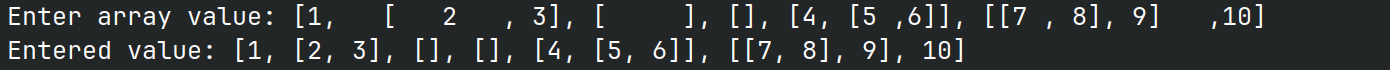
\includegraphics[width=.9\textwidth]{\reportDirectory/parsing.png}
    \caption{Приклад складного варіанту для парсингу}
    \label{fig:task}
\end{figure}


\newpage
\subsection{Відображення \textit{ParsedVec}}
Додамо можливість виводити нашу структуру \textit{ParsedVec}.
Для цього реалізуємо trait Display для нашої структури \textit{ParsedVec}.
\begin{lstlisting}[language=Rust, style=colouredRust]
impl<T: Display> Display for ParsedItem<T> {
    fn fmt(&self, f: &mut fmt::Formatter<'_>) -> fmt::Result {
        match self {
            ParsedItem::Value(val) => write!(f, "{}", val),
            ParsedItem::NestedVec(vec) => write!(f, "{}", vec),
            _ => Ok(()),
        }
    }
}

impl<T: Display> Display for ParsedVec<T> {
    fn fmt(&self, f: &mut fmt::Formatter<'_>) -> fmt::Result {
        let content: String = self
            .0
            .iter()
            .map(|item| item.to_string())
            .collect::<Vec<String>>()
            .join(", ");
        write!(f, "[{}]", content)
    }
}
\end{lstlisting}


\newpage
\subsection{Бітове подання \textit{ParsedVec}}
І на кінець реалізуємо наш trait ShowBytes для нашої структури \textit{ParsedVec}.
Для трохи кращої читаємості приберемо зайву інформацію.
\begin{lstlisting}[language=Rust, style=colouredRust]
fn print_layers(layers: &Vec<bool>) {
    let s: String = layers
        .iter()
        .map(|l| match l {
            true => "│   ",
            false => "    ",
        })
        .collect();
    print!("{}", s);
}

fn show_bytes_vec<T: Display + ShowBytes>(vec: &Vec<T>, layers: &Vec<bool>) {
    print_layers(layers);
    println!("│{{");
    print_layers(layers);
    print!("│    addr: {:p} (", vec);
    let addr = vec as *const Vec<T> as usize;
    print_raw_bytes(addr, 8);
    println!(")");

    print_layers(layers);
    print!("│    capacity: {} (\x1b[34m", vec.capacity());
    vec.capacity().show_bytes();
    println!("\x1b[0m)");

    print_layers(layers);
    print!("│    length: {} (\x1b[32m", vec.len());
    vec.len().show_bytes();
    println!("\x1b[0m)");

    print_layers(layers);
    print!("│    ptr: \x1b[31m");
    (vec.as_ptr() as usize).show_bytes();
    println!("\x1b[0m");

    print_layers(layers);
    println!("│}}");
}

impl<T: ShowBytes + Display> ParsedItem<T> {
    pub fn show_bytes_(&self, layers: &mut Vec<bool>) {
        match self {
            ParsedItem::Value(val) => {
                println!("Value:");
                print_layers(layers);
                println!("│{{");
                print_layers(layers);
                print!("│    addr: {:p} (", val);
                let addr = val as *const T as usize;
                print_raw_bytes(addr, 8);
                println!(")");

                print_layers(layers);
                print!("│    bin: ");
                let ptr = val as *const T as usize as *const u8;
                let size = size_of::<ParsedItem<T>>();
                print_bytes(ptr, size);
                println!();

                print_layers(layers);
                println!("│    value: {val}");

                print_layers(layers);
                println!("│}}");
            }
            ParsedItem::NestedVec(vec) => {
                vec.show_bytes_(layers);
            }
        }
    }
}

impl<T: ShowBytes + Display> ShowBytes for ParsedItem<T> {
    fn show_bytes(&self) {
        self.show_bytes_(&mut Vec::new());
    }
}

impl<T: ShowBytes + Display> ParsedVec<T> {
    fn propagate_show_tree(&self, layers: &mut Vec<bool>) {
        let len = self.0.len();
        let mut inner_layers = layers.clone();
        inner_layers.push(true);

        for i in 0..(len - 1) {
            print_layers(&inner_layers);
            println!();
            print_layers(layers);
            print!("├───");
            self.0[i].show_bytes_(&mut inner_layers);
        }

        let level = inner_layers.len();
        print_layers(&inner_layers);
        inner_layers[level - 1] = false;
        println!();
        print_layers(layers);
        print!("└───");
        self.0[len - 1].show_bytes_(&mut inner_layers);
    }
    pub fn show_bytes_(&self, layers: &mut Vec<bool>) {
        if layers.is_empty() {
            println!("Vec");
        } else {
            println!("NestedVec");
        }

        show_bytes_vec(&self.0, layers);

        if self.0.is_empty() {
            return;
        }

        self.propagate_show_tree(layers);
    }
}

impl<T: ShowBytes + Display> ShowBytes for ParsedVec<T> {
    fn show_bytes(&self) {
        self.show_bytes_(&mut Vec::new());
    }
}
\end{lstlisting}

\newpage
\noindent
Як приклад давайте наведемо двовимірний масив
\begin{figure}[h!]
    \centering
    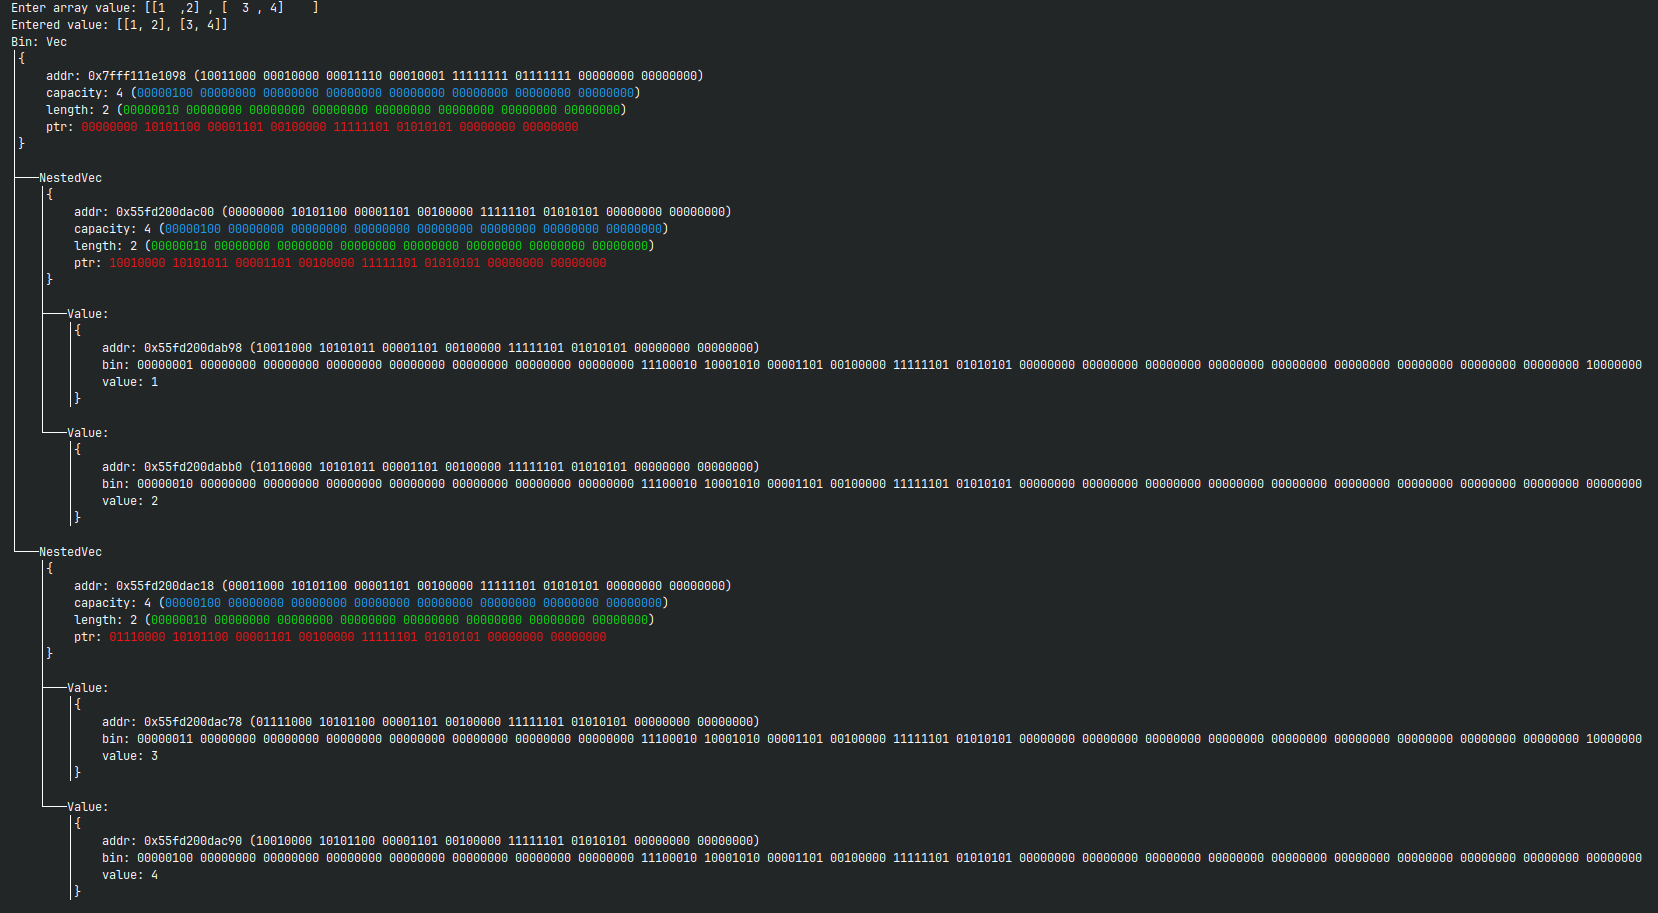
\includegraphics[width=\textwidth]{\reportDirectory/res.png}
    \caption{Представлення \textit{ParsedVec} у памяті}
    \label{fig:task}
\end{figure}


\newpage
\section{Висновки}
В ході виконання лабораторної робити було розглянуто подання різних типів даних в пам'яті, а також подання n-вимірного масиву в пам'яті. 
